
\section{Introduction}

Peer-sampling
protocols~\cite{voulgaris2005cyclon,jelasity2007gossip,tolgyeski2009adaptive}
constitute a fundamental mechanism for a number of large-scale
distributed applications both on the Cloud~\cite{decandia2007dynamo}
and in a peer-to-peer
setting~\cite{Frey09Middleware,voulgaris2005sub,wuhib2009robust}. By
providing each node with a continuously changing partial view of the
network, they make applications resilient to churn~\cite{bertier-d2ht}
and inherently load balancing~\cite{Frey09DSN}. In the context of
video streaming, for example, a peer-sampling protocol makes it
possible to distribute the streaming load over all peers without
requiring the creation and the maintenance of rigid structures like
multiple trees~\cite{Frey09DSN, monod:THESIS}.  

% made browser-to-browser communications easy even
% within complex network environments that involve firewalls, proxies,
% Net Address Translation (NAT) and mobile networks. A simple click on a
% http link in the browser launches a browser-based video-conferencing
% application as in Firefox Hello, a torrent download browser-based application as in
% webtorrent~\cite{webtorrent}, or a decentralized collaborative
% real-time editor as in CRATE~\cite{nedelec2016crate}. Browsers can be
% seen as an application containter and WebRTC as a communication layer
% for distributed applications deployed in browsers. Users start an
% application in their browsers, create a session URL to allow remote
% access and notify other users. Remote participants have just to click
% on this link to deploy the application in their browsers and join the session.

% Many large scale distributed applications relies on gossip-based peer
% sampling protocols such as \CYCLON~\cite{voulgaris2005cyclon} to
% enable information dissemination~\cite{eugster2003lightweight,
%   tolgyeski2009adaptive}, aggregation~\cite{jelasity2004epidemic} or
% network management~\cite{jelasity2009tman, voulgaris2005epidemic}.


The recent introduction of WebRTC~\cite{webrtc} has renewed the
research interest in a variety of applications that require
peer-sampling protocols such as video streaming~\cite{hivejs,smoothcache2},
content-delivery networks~\cite{Zhang:2013:MBC:2465351.2465379}, or
real-time collaborative editors~\cite{nedelec2016crate}. However,
deploying existing peer-sampling protocols on top of WebRTC raises
important technical challenges.
\begin{inparaenum}[(1)]
\item WebRTC does not manage addressing nor routing; this makes
  connection establishement much more costly than on IP networks and
  more likely to fail. 
\item Browsers run on desktops, laptops and mobile phones. This
  requires protocols that reduce resource consumption as much as
  possible.
\item The ability to launch WebRTC sessions through simple HTTP links
  exposes applications to sudden bursts of popularity.  % Suppose
  % massive online lecture platforms allow students to share their
  % notes. Many lectures run in parallel involving various number of
  % students, i.e., from few to thousands. Also, even during the
  % editing
  % session the audience is subject to significant changes in size,
  % going from thousands to hundreds.
\end{inparaenum}
Consider the example of a user who is streaming a video directly from
his mobile phone to some of his friends. The user suddenly witnesses
some dramatic event, and his friends spread the news by twitting the
stream's address. Instantly a huge number of users connect and start
watching the stream on their laptops and phones. The streaming
mechanisms, and the protocols it relies on must be able to adapt to
this sudden burst of popularity, maintaining their quality of service,
while being able to return to their initial configuration when the
popularity burst subsides. 

% Publishing the
%   link to a WebRTC video stream on Twitter can create the buzz and
%   generate massive joins for an unpredictable period of time.

Unfortunately, existing peer-sampling protocols
% Pascal: IMHO not useful here
%, which lie at the bases of several video streaming
%solutions~\cite{Frey09Middleware,Abeni2009,smoothcache20} 
lack this capability. On the one hand, \SCAMP~\cite{ganesh2003peer}
features some form of adaptation but falls short in the context of
WebRTC applications. \SCAMP maintains partial views of size
$\log(n)+k$, $n$ being the number of nodes, and $k$ being a
constant. But its connection establishment process based on random
walks cannot handle the connection failures that often occur in
WebRTC. On the other hand, the most popular approaches like
\CYCLON~\cite{voulgaris2005cyclon} and the whole RPS protocol
family~\cite{jelasity2007gossip} provide application nodes with
fixed-size views of the network based on parameters that have to be
configured at deployment time. This forces developers to oversize
partial views to handle potential bursts, either wasting resources, or
not provisioning for large-enough settings.
%  Unfortunatly, deploying Scamp on
% top of WebRTC fails due to the connection estabilishement failures of
% WebRTC. Another approach is just to oversize partial views and use
% protocol as Cyclon~\cite{voulgaris2005cyclon}. Unfortunatly, this
% approach consumes more ressources and create and renew periodically
% more connections than required. With this approach, small networks
% will end up paying the price of the largest one. It does not also
% provide a way to compute a fan-out that will ensure high delivery rate
% in any situation.
To address this problem, it would in principle be possible to estimate
the real number of network nodes by periodically running an
aggregation protocol~\cite{montresor2004robust}, and by reconfiguring
\CYCLON, or other RPS solutions based on this. However, this aggregation
protocol would have to run quite frequently, resulting in significant
network overhead to anticipate a popularity burst that may never
happen.

% The scientific challenge consists in finding a way to adapt to the
% network size without actually measuring its number of members as
% proposed by Scamp, but running on top of WebRTC.

%% FORCE POSITIONNING
\begin{figure*}
\centering
\subfloat[Figure A][\label{fig:webrtcA}
$p_1$ connects to $p_2$ using the signaling service. 
1: $p_1$ pushes its offer ticket; 
2: $p_2$ pulls the ticket; 
3: $p_2$ pushes its response; 
4: $p_1$: pulls the response and establishes a 
connection with $p_2$. $p_3$ does the same with $p_2$. 
%%Figure~\ref{fig:webrtcB} depicts the resulting network.
]{
  
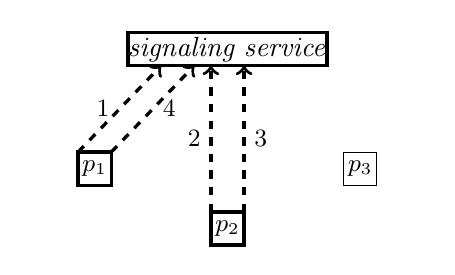
\begin{tikzpicture}[scale=1.2]

\newcommand\X{40pt};
\newcommand\Y{18pt};

\draw( 1.5*\X, 0); %% spacing
\draw(-1.5*\X, 0); %% spacing

\draw[fill=white,very thick](0*\X, 0*\Y) 
node{\emph{signaling service}} +(-30pt,-5pt) rectangle +(30pt,5pt);

\small
\draw[->,dashed, very thick](-5 -1*\X, 5-2*\Y) --
node[anchor=east]{1} (-20pt,-5pt);
\draw[->,dashed, very thick]( 5 -1*\X, 5-2*\Y) --
node[anchor=west]{4} (-10pt,-5pt);

\draw[->,dashed, very thick](-5pt,  5-3*\Y) --
node[anchor=east]{2}(-5pt,-5pt);
\draw[->,dashed, very thick](5pt , 5-3*\Y) --
node[anchor=west]{3} (5pt,-5pt);


\draw[fill=white, very thick]
(-1*\X,-2*\Y) node{$p_1$} +(-5pt,-5pt) rectangle +(5pt,5pt);
\draw[fill=white, very thick]
(0*\X, -3*\Y) node{$p_2$} +(-5pt,-5pt) rectangle +(5pt,5pt);
\draw[fill=white] (1*\X, -2*\Y) node{$p_3$} +(-5pt,-5pt) rectangle +(5pt,5pt);

\end{tikzpicture}

% \begin{tikzpicture}
% \matrix (m) [matrix of math nodes,row sep=4em,column sep=4em] {
% \node(ss)[draw]{signaling}; & \node(p3)[draw]{p3}; \\
% \node(p1)[draw]{p1}; & \node(p2)[draw]{p2}; \\
% };
% \path[->]
%   (p2) edge[dashed] node[fill=white]{1:emit} (ss)
%   (p3) edge[dashed] node[fill=white,bend left]{2:pull} (ss)
%   (p3) edge[dashed, bend right] node[fill=white]{3:accept} (ss)
%   (p2) edge[dashed,bend left] node[fill=white]{4:pull} (ss)
%   (p3) edge[<->,thick] node[fill=white,right]{5:connected} (p2);
% \end{tikzpicture}}
\hspace{5pt}
\subfloat[Figure B][\label{fig:webrtcB}
$p_1$ connects to $p_3$ using $p_2$ as mediator. 
1: $p_1$ sends its offer ticket to $p_2$; 
2: $p_2$ forwards it to $p_3$ and registers $p_1$ as the emitter; 
3: $p_3$ sends its response to $p_2$; 
4: $p_2$ forwards it to the emitter $p_1$ which connects to $p_3$.]{
  
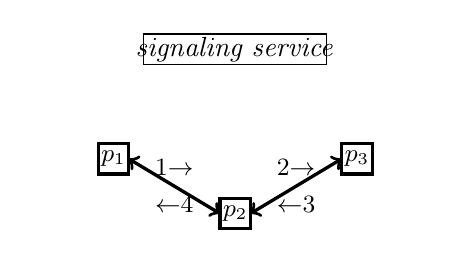
\begin{tikzpicture}[scale=1.1]

\newcommand\X{40pt};
\newcommand\Y{18pt};

\draw(1.7*\X, 0); %% spacing
\draw(-1.7*\X, 0); %% spacing

\draw[fill=white](0*\X, 0*\Y)
node{\emph{signaling service}} +(-30pt,-5pt) rectangle +(30pt,5pt);

\small
\draw[<->, very thick](5-1*\X,-2*\Y)--
node[anchor=south]{1$\rightarrow$}
node[anchor=north]{$\leftarrow$4}(-5pt,-3*\Y);
\draw[<->, very thick](5pt,-3*\Y)--
node[anchor=south]{2$\rightarrow$}
node[anchor=north]{$\leftarrow$3}(-5+1*\X,-2*\Y);

\draw[fill=white, very thick]
(-1*\X,-2*\Y) node{$p_1$} +(-5pt,-5pt) rectangle +(5pt,5pt);
\draw[fill=white, very thick]
(0*\X, -3*\Y) node{$p_2$} +(-5pt,-5pt) rectangle +(5pt,5pt);
\draw[fill=white, very thick]
(1*\X, -2*\Y) node{$p_3$} +(-5pt,-5pt) rectangle +(5pt,5pt);

\end{tikzpicture}

% \begin{tikzpicture}
% \matrix (m) [matrix of math nodes,row sep=4em,column sep=4em] {
% \node(ss)[draw]{signaling}; & \node(p3)[draw]{p3}; \\
% \node(p1)[draw]{p1}; & \node(p2)[draw]{p2}; \\
% };
% \path[->]
%   (p1) edge[dashed,bend left] node[fill=white]{1:emit} (p2)
%   (p2) edge[dashed,bend left] node[fill=white,left]{2:emit/p1} (p3)
%   (p3) edge[dashed,bend left] node[fill=white,right]{3:accept/p1} (p2)
%   (p2) edge[dashed,bend left] node[fill=white]{4:accept} (p1)
%   (p1) edge[<->,thick] (p2)
% %  (p1) edge[<->,thick,bend left] (p3)
%   (p2) edge[<->,thick]  (p3);

% \end{tikzpicture}}
\hspace{5pt}
\subfloat[Figure C][\label{fig:webrtcC}
The resulting network overlay: a fully connected network composed of
3 members.]{
  
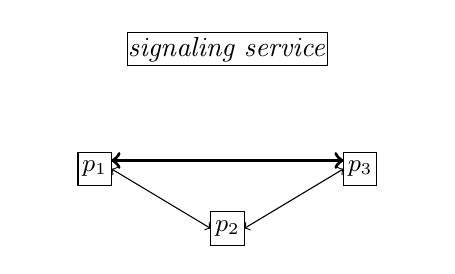
\begin{tikzpicture}[scale=1.2]

\newcommand\X{40pt};
\newcommand\Y{18pt};

\draw(1.5*\X, 0); %% spacing
\draw(-1.5*\X, 0); %% spacing

\draw[fill=white](0*\X, 0*\Y)
node{\emph{signaling service}} +(-30pt,-5pt) rectangle +(30pt,5pt);

\small
\draw[<->](5-1*\X,-2*\Y)--(-5pt,-3*\Y);
\draw[<->](5pt,-3*\Y)--(-5+1*\X,-2*\Y);
\draw[<->, very thick](5 - 1*\X, 2.5 -2*\Y)--(-5+1*\X, 2.5 -2*\Y);

\draw[fill=white]
(-1*\X,-2*\Y) node{$p_1$} +(-5pt,-5pt) rectangle +(5pt,5pt);
\draw[fill=white]
(0*\X, -3*\Y) node{$p_2$} +(-5pt,-5pt) rectangle +(5pt,5pt);
\draw[fill=white]
(1*\X, -2*\Y) node{$p_3$} +(-5pt,-5pt) rectangle +(5pt,5pt);

\end{tikzpicture}


% \begin{tikzpicture}
% \matrix (m) [matrix of math nodes,row sep=4em,column sep=4em] {
% \node(ss)[draw]{signaling}; & \node(p3)[draw]{p3}; \\
% \node(p1)[draw]{p1}; & \node(p2)[draw]{p2}; \\
% };
% \path[->]
%   (p1) edge[<->,thick] (p2)
%   (p1) edge[<->,thick] (p3)
%   (p2) edge[<->,thick]  (p3);
% \end{tikzpicture}}
\caption{\label{fig:webrtc}Creating an overlay network on top of WebRTC.}
\end{figure*}


In this paper, we address the challenge of a dynamically adaptive
peer-sampling, by introducing \SPRAY, a novel random peer-sampling
protocol inspired by both \SCAMP~\cite{ganesh2003peer} and
\CYCLON~\cite{voulgaris2005cyclon}. \SPRAY improves the
state-of-the-art in several ways.
\begin{inparaenum}[(i)]
\item It dynamically adapts the neighborhood of each peer. Thus, the
  number of connections scales logarithmically with the network size.
\item It only uses neighbor-to-neighbor interactions to establish
  connections. Thus, the process takes constant time.
\item It quickly converges to a topology with properties similar to
  those of random graphs. Thus, the network becomes robust to massive
  failures, quickly disseminates information etc.
\item Experiments show the flexibility of \SPRAY and highlight its
  efficiency improvements at the cost of little overhead.
\end{inparaenum}

\SPRAY not only relieves developers from having to foresee the number
of users of their distributed applications, but most importantly it
allows applications to adapt to sudden burst in popularity. We
demonstrate the effectiveness of \SPRAY by simulation in the context
of a large-scale flash-crowd scenario, as well as on a real use case
using \CRATE~\cite{nedelec2016crate}, deployed on Grid'5000. Our
results demonstrate that \SPRAY significantly reduces network traffic
with respect to a standard peer-sampling protocol, while adapting to
the current size of the network.

% , a real-time decentralized editor directly
% running in web browsers, thus on laptops, tablets, or mobile
% phones. We experiment with \CRATE by deploying 600 editors on

The rest of this paper is organized as follows: Section~\ref{sec:relatedwork}
reviews the related work. Section~\ref{sec:problem} states the scientific
problem. Section~\ref{sec:proposal} details the \SPRAY
protocol. Section~\ref{sec:experimentation} presents experimentation results of
\SPRAY and compares them to state-of-the-art. Section~\ref{sec:use-case} details
our experiment with \CRATE, a real-time collaborative editor running in
browsers. We conclude in Section~\ref{sec:conclusion}.




%%% Local Variables:
%%% mode: latex
%%% TeX-master: "../paper"
%%% End:
